\hfil
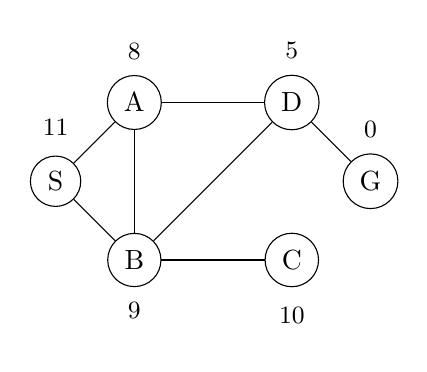
\begin{tikzpicture}
    \begin{scope}[grow'=right,
        every node/.style = {shape=circle, draw, align=center},
        every tree node/.style={anchor=base west}]
        \node[label={\small 11}] (S) at (0,0) {S};
        \node[label={\small 8}] (A) at (1,1) {A};
        \node[label=below:{\small 9}] (B) at (1,-1) {B};
        \node[label=below:{\small 10}] (C) at (3,-1) {C};
        \node[label={\small 5}] (D) at (3,1) {D};
        \node[label={\small 0}] (G) at (4,0) {G};
    \end{scope}

    \begin{scope}
    \path [-] (S) edge node {} (A);
    \path [-] (S) edge node {} (B);
    \path [-] (A) edge node {} (B);
    \path [-] (B) edge node {} (C);
    \path [-] (A) edge node {} (D);
    \path [-] (B) edge node {} (D);
    \path [-] (D) edge node {} (G);
    \end{scope}

  \end{tikzpicture}